\documentclass[12pt]{exam}
\usepackage[hon]{template-for-exam}
\footer{}{}{}
\header{}{}{}

\usepackage{tikz,graphicx}
\usetikzlibrary{shadings,decorations.pathmorphing,arrows.meta,patterns}

\shadedsolutions
\printanswers

\def\mystrut{\protect\rule[-2.2ex]{0ex}{2.2ex}} 
\qformat{ \textbf{Task \#\thequestion}
  \ifthenelse{\equal{\thequestion}{\thequestiontitle}}
    {}
    {: \emph{\thequestiontitle}}
  \mystrut  \hfill}

\begin{document}
\begin{questions}

\Large

\question Write down a few words or equations to explain each of Newton's Laws of Motion.

\vs \hrule \vs

\question You ($m=46$ kg) are standing on a an elevator on the top floor of a building.  The elevator begins to go down towards the ground floor and does so by accelerating downward at 2.7 m/s$^2$.  What is the normal force acting on you?

\begin{solution}[\stretch{1}]
  326.6 N 
\end{solution}

\hrule \vs

\question Two crates of mass 65~kg and 125~kg are in contact and at rest on a horizontal frictionless surface.  A 650-N force is exerted on 65-kg crate.  Calculate (a) the acceleration of the system and (b) the force that each crate exerts on the other.

\begin{solution}[\stretch{1}]
  (a) \SI{3.42}{m/s^2} (b) \SI{427.5}{N} (c) \SI{3.42}{m/s^2} and \SI{22.3}{N} 
\end{solution}


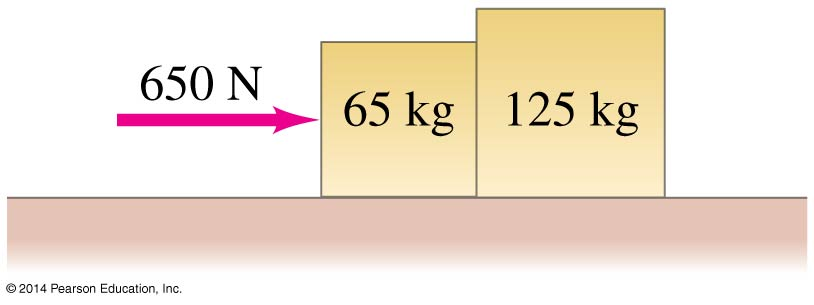
\includegraphics[height=3cm]{OpenStaxImages/Giancolli4-57.jpg}

\vspace{1em}

{\small Based on chapter 4, problem 49, in Giancolli \emph{Physics: Principles with Application}, 7th ed. }



\end{questions}
\end{document}